\documentclass[oneside,final,14pt,a4paper]{extreport}

%=====================================================================
%  BACHELOR THESIS PROPOSAL
%  1 Introduction and research problem
%  2 Research question
%  3 Novelty and contributions
%  4 State-of-the-Art
%  5 Goal of the Thesis
%  6 Detailed Work Plan and schedule
%  7 References
%=====================================================================

%---------------------------------------------------------------------
% Fonts and encoding
%---------------------------------------------------------------------
\usepackage[T1]{fontenc}           
\usepackage[utf8]{inputenc}
\usepackage[english]{babel}
\usepackage{tempora}                % Times New Roman alike font

%%%%% ADDED TO SUPPORT TT BOLD FACES %%%%
\DeclareFontShape{OT1}{cmtt}{bx}{n}%
  {<5><6><7><8><9><10><10.95><12><14.4><17.28><20.74><24.88>cmttb10}{}
\renewcommand{\ttdefault}{pcr}
%%%%% END %%%%%%%%%%%%%%%%%%%%%%%%%%%%%%%

%---------------------------------------------------------------------
% Page layout
%---------------------------------------------------------------------
\usepackage{vmargin}
\setpapersize{A4}
\setmarginsrb{2.5cm}{2.2cm}{2.2cm}{2.2cm}{0pt}{10mm}{0pt}{13mm}
\usepackage{setspace}
\setstretch{1.5}
\usepackage{indentfirst}
\parindent=1.25cm

%---------------------------------------------------------------------
% Mathematics and theorems
%---------------------------------------------------------------------
\usepackage{amsmath,amsfonts}
\usepackage{amsthm}
\usepackage{upgreek}
\usepackage{bm}

\newtheorem{theorem}{Theorem}
\newtheorem{corollary}{Corollary}
\newtheorem{lemma}{Lemma}
\newtheorem{proposition}{Proposition}
\theoremstyle{definition}
\newtheorem{definition}{Definition}
\theoremstyle{remark}
\newtheorem*{remark}{Remark}
\newtheorem*{example}{Example}

%---------------------------------------------------------------------
% Colour, graphics, tables, lists
%---------------------------------------------------------------------
\usepackage{xcolor}                 % was "color"; tikz needs xcolor
\usepackage{graphicx}
\graphicspath{{figs/}}              % path to images
\usepackage{float}
\usepackage{array}
\usepackage{multirow}               % was loaded twice -> once
\usepackage{booktabs}
\usepackage{longtable}
\usepackage[font=singlespacing,labelfont=bf]{caption} % was loaded twice -> once
\usepackage{subcaption}
\usepackage{enumitem}
\newlist{inlinelist}{enumerate*}{1}
\setlist*[inlinelist,1]{label=(\arabic*)}

%---------------------------------------------------------------------
% TikZ  (was MISSING: needed by the system architecture diagram)
%---------------------------------------------------------------------
\usepackage{tikz}
\usetikzlibrary{positioning,arrows.meta}

%---------------------------------------------------------------------
% Bibliography (natbib removed: conflicts with biblatex)
%---------------------------------------------------------------------
\usepackage{csquotes}
\usepackage[backend=biber,style=ieee,autocite=inline]{biblatex}
\addbibresource{references.bib}     % replaces deprecated \bibliography{...}
\DefineBibliographyStrings{english}{%
  bibliography = {References},}

%---------------------------------------------------------------------
% Miscellaneous
%---------------------------------------------------------------------
\usepackage{chngcntr}
\usepackage{pdfpages}
\usepackage{atbegshi,picture}
\usepackage{url}
\usepackage{placeins}               % for \FloatBarrier
\usepackage{fancyhdr}
% \usepackage{blindtext}            % optional dummy text

%---------------------------------------------------------------------
% Captions, counters, headers
%---------------------------------------------------------------------
\captionsetup[table]{labelfont={normalfont}, name={TABLE}, labelsep={newline}}
\DeclareCaptionLabelSeparator{figSep}{.\quad}
\captionsetup[figure]{labelfont={normalfont}, name={Fig.}, labelsep=period}

% No \chapter is used, but report classes define
% \thesection = \thechapter.\arabic{section} -> sections would show as 0.1, 0.2...
\renewcommand{\thesection}{\arabic{section}}
\counterwithin{figure}{section}
\counterwithin{table}{section}
\counterwithin{equation}{section}
\setcounter{secnumdepth}{3}         % number subsubsections (metrics)

%Hints
\newcommand\pic[1]{(Fig.~\ref{#1})} % Ref on figure
\newcommand\tab[1]{(Tab.~\ref{#1})} % Ref on table

\setlength{\headheight}{32.0976pt}

\newenvironment{bottompar}{\par\vspace*{\fill}}{\clearpage}

\newcommand{\dedication}[1]
   {\thispagestyle{empty}
   \begin{flushleft}\raggedleft #1\end{flushleft}
}

\pagestyle{fancyplain}

\renewcommand{\chaptermark}[1]%
   {\markboth{\chaptername~\thechapter~--~#1}{}}
\renewcommand{\sectionmark}[1]%
   {\markright{\thesection\ #1}}

\rhead[\fancyplain{}{\bf\leftmark}]%
      {\fancyplain{}{\bf\thepage}}
\lhead[\fancyplain{}{\bf\thepage}]%
      {\fancyplain{}{\bf\rightmark}}
\cfoot{}

%---------------------------------------------------------------------
% hyperref: loaded ONCE and last
%---------------------------------------------------------------------
\usepackage{hyperref}
\hypersetup{colorlinks=true, linkcolor=black, citecolor=black, urlcolor=black}

%---------------------------------------------------------------------
% Title
%---------------------------------------------------------------------
\title{Confidence-Aware Adaptive Verification of LLM Recommendations\\
in Introductory Programming Tasks}
\author{Lidia Davydova\\[1mm]Supervisor: Paolo Ciancarini}   % TODO: fill in
\date{\today}

%=====================================================================
\begin{document}
\maketitle

%=====================================================================
\section{Introduction and Research Problem}
%=====================================================================

\subsection{Context and Motivation}
Large language models (LLMs) are increasingly used in programming education and
software engineering: they generate code, explain programs, debug errors, and
propose answers to programming tasks \cite{Ma2023,Cambaz2024}. At the same
time, these systems can produce plausible but incorrect outputs, so the quality
of the joint human--AI outcome depends not only on the accuracy of the model
but also on whether the user relies on it \emph{appropriately}, i.e., accepts
correct recommendations and rejects incorrect ones. Accepting incorrect
recommendations is commonly described as over-reliance; rejecting correct
recommendations as under-reliance \cite{PoursabziSangdeh2021,Vasconcelos2023}.

Verification support can help users evaluate LLM recommendations. Programming
tasks are particularly suitable for such support because independent evidence
can often be produced objectively through execution, tests, traces, or
counterexamples. However, providing verification on every trial may introduce
unnecessary interaction cost, and prior work shows that simply providing more
information (e.g., AI explanations) does not automatically reduce over-reliance
\cite{Bucinca2021,Vasconcelos2023}.

Prior work also suggests that the usefulness of explanations depends on whether
users can understand and connect the explanation to the AI's prediction. When
explanations are difficult to interpret or map to the recommendation, they may
provide little additional assistance over prediction-only baselines
\cite{ma2024arereallysureunderstanding}. More generally, producing human-interpretable explanations remains a challenge for explainable AI. This motivates the use of verification evidence
that is independent of the LLM's own explanation rather than relying on an
additional AI-generated justification.

Programming tasks provide a suitable setting for studying such verification.
For many introductory programming problems, correctness can be independently
checked through program execution, test cases, execution traces, or
counterexamples. These forms of evidence are directly grounded in the task
itself and do not require the participant to assess the quality of another
LLM-generated explanation. Therefore, programming tasks allow the study to
isolate the effect of access to independent verification evidence on reliance
on an LLM recommendation.

\subsection{Research Problem}
The research problem is how to provide verification support \emph{selectively},
based on information that is available before the correctness of the LLM
recommendation is known. This thesis investigates whether a simple adaptive
policy based primarily on the user's initial confidence can selectively provide
independent verification support while maintaining appropriate reliance on LLM
recommendations.

The study focuses on a simple and interpretable adaptive policy rather than
developing a new LLM, a new verification algorithm, or an optimization method.

%=====================================================================
\section{Research Question}
%=====================================================================

\textbf{How does confidence-aware adaptive verification affect reliance on LLM
recommendations in introductory programming tasks compared with static and no
verification?}

The main research question is decomposed into three secondary research
questions:

\begin{description}[leftmargin=2.5cm,style=nextline]
    \item[RQ1.] How do no verification, static verification, and adaptive
    verification affect final answer accuracy, over-reliance, and
    under-reliance?

    \item[RQ2.] Can adaptive verification achieve comparable reliance and accuracy
outcomes to static verification while requiring less verification support and
lower verification cost?

    \item[RQ3.] How does the effectiveness and verification cost of the adaptive
policy differ across levels of initial user confidence and programming task
types?
\end{description}

In addition, a policy premise check examines whether initial confidence is
associated with initial answer correctness, supporting the interpretation of
the adaptive condition (Section~\ref{subsec:premise}).

%=====================================================================
\section{Novelty and Contributions}
%=====================================================================

The novelty of the thesis is \emph{not} the observation that human confidence
relates to reliance on AI --- this link is well documented
\cite{ToRelyOrNotToRely2024} and is taken here as a premise. The novelty lies
in combining three elements that have mostly been studied in isolation:
\begin{enumerate}
    \item confidence-sensitive \emph{adaptive} support, in which the user's
    initial confidence is used as a per-trial \emph{trigger} that decides
    \emph{when} support is displayed, rather than being an outcome to be
    calibrated or a signal derived from AI-side uncertainty;
    \item \emph{independent, execution-based} verification evidence (test
    results, traces, counterexamples) rather than additional AI-generated
    explanations or confidence scores;
    \item a programming task setting, in which recommendations can be validated
    in advance and verification evidence can be produced objectively.
\end{enumerate}

In addition, the thesis explicitly evaluates the cost--quality trade-off,
i.e., whether comparable reliance and accuracy outcomes can be achieved with
fewer interventions. This perspective is consistent with the argument that AI
evaluation should measure not only correctness, but also the cost of verifying
whether an AI output can be safely trusted
\cite{ToRelyOrNotToRely2024,VerificationCost2026}.

The thesis is expected to make the following contributions:
\begin{enumerate}
    \item \textbf{Empirical evidence} on whether a simple confidence-based
    policy can achieve reliance and accuracy outcomes comparable to static
    verification while displaying verification on fewer trials (RQ1--RQ3).
    \item \textbf{A validated benchmark} of 18 introductory Python programming
    tasks with fixed, pre-validated LLM recommendations, task-type and
    difficulty labels, and task-specific verification data.
    \item \textbf{A reproducible experimental prototype} implementing the three
    conditions (no verification, static verification, adaptive verification)
    with complete trial logging.
    \item \textbf{An analysis pipeline} computing accuracy, over-reliance,
    under-reliance, appropriate reliance, verification rate, decision-change
    rate, and verification efficiency.
\end{enumerate}

The contribution is deliberately \emph{not} a new LLM, a new verification
algorithm, or a general-purpose adaptive tutoring system. Instead, the thesis
provides a controlled, reproducible human--AI interaction experiment together
with the infrastructure (benchmark, prototype, policy, and analysis pipeline)
required to reproduce and evaluate this experimental approach.

%=====================================================================
\section{State-of-the-Art}
%=====================================================================

\subsection{Appropriate Reliance and Miscalibration}
A central problem in human--AI decision-making is not simply whether users
trust an AI system, but whether they rely on it appropriately. Appropriate
reliance means accepting correct recommendations and rejecting incorrect ones.
When users accept incorrect recommendations, this is commonly described as
over-reliance; when users reject correct recommendations, this is under-reliance
\cite{PoursabziSangdeh2021}.

Prior research shows that reliance on AI recommendations is affected by system
reliability, the nature of the task, and user characteristics. In practice,
human--AI interaction can therefore fail not only because an AI system is
inaccurate, but also because users do not calibrate their reliance to the
quality of the recommendation \cite{PoursabziSangdeh2021,Vasconcelos2023}.

\subsection{Verification and Cognitive Forcing}
One way to reduce inappropriate reliance is to introduce mechanisms that
encourage users to engage more critically with AI advice. Cognitive forcing
functions are a related design approach: they require the user to slow down,
deliberate, or inspect evidence before accepting an AI recommendation
\cite{Bucinca2021}.

Research also shows that explanations alone do not necessarily prevent
over-reliance. Users may still accept incorrect advice even when additional
information is provided, especially if that information is not sufficiently
diagnostic or independent of the AI recommendation itself \cite{Vasconcelos2023}.
This makes verification support, rather than another AI explanation, a
promising intervention.

Recent work has argued that correctness alone is insufficient for evaluating
the reliability of AI systems. In practical settings, users must verify model
outputs before relying on them, and this verification process consumes time,
attention, cognitive effort, and sometimes computational resources
\cite{VerificationCost2026}. Consequently, an AI system that achieves high
accuracy but produces outputs that are difficult or expensive to verify may be
less useful than a slightly less accurate system whose errors can be detected
quickly. This perspective motivates treating verification cost as a first-class
evaluation dimension rather than as an incidental usability measure.

The present thesis operationalises this perspective in an introductory
programming setting. Verification cost is approximated by the frequency with
which verification support must be displayed, together with the participant's
response time and decision-change behaviour. The adaptive policy is therefore
not evaluated only by whether it improves final accuracy, but also by whether
it can preserve appropriate reliance while reducing the amount of verification
support required.

\subsection{Self-Confidence Calibration and Adaptive Support}
Closest to this thesis is work that uses a person's own confidence in
human--AI decision-making. \cite{ToRelyOrNotToRely2024} show that
discrepancies between initial self-confidence and actual correctness are
systematically associated with inappropriate reliance on AI recommendations
and propose \emph{calibrating} human self-confidence to improve appropriate
reliance. Related work similarly tailors support to the user's trust or
confidence state \cite{Xie2025AdjustForTrust}.

These studies differ from the present thesis in three respects. First, they
treat confidence as an \emph{outcome to be corrected}: the intervention aims
to change the user's internal state and is applied on every trial. Here,
confidence is an \emph{input signal}: a lightweight trigger that determines
\emph{when} external support is displayed, leaving the user's confidence
itself unchanged. Second, prior support consists of AI-generated confidence
scores, explanations, or calibration feedback, whereas this thesis provides
\emph{independent, execution-based} verification evidence (tests, traces,
counterexamples) that is not derived from the LLM recommendation. Third,
prior evaluations use estimation tasks such as income prediction, where
ground-truth evidence cannot be shown at decision time; introductory
programming tasks make objective verification evidence directly available.
Their central finding is taken here as a premise: if initial confidence
carries diagnostic signal, it can also be used to decide \emph{when}
verification support is worth its interaction cost. This cost dimension,
absent from calibration-oriented work, is a primary outcome of the present
study (RQ2).

\subsection{LLM Assistance in Programming}
LLMs are increasingly used in software engineering and programming education,
including code generation, debugging, and explanation tasks
\cite{Ma2023,Cambaz2024}. At the same time, these systems can produce plausible
but incorrect outputs, which creates a need for users to critically evaluate
recommendations rather than accept them at face value.

Programming tasks are a useful domain for studying verification because
independent evidence can often be produced through execution, tests, traces, or
counterexamples. This makes it possible to separate the recommendation from the
verification mechanism and experimentally study how users respond to each.

\subsection{Research Gap}
Prior work has shown that user confidence, trust calibration, and
verification-related cues influence reliance on AI recommendations, and that
explanation-based interventions may reduce over-reliance, but their
effectiveness depends on the task, the interface, and the cost of engaging with
the support \cite{Vasconcelos2023}. However, less is known about whether a
participant's initial confidence can be used as a lightweight trigger for
selectively displaying \emph{independent verification evidence} after an LLM
recommendation in introductory programming tasks. This motivates the focus of
the present study on verification support that is independent of the LLM
recommendation and selectively displayed through a confidence-aware policy.

%=====================================================================
\section{Goal of the Thesis}
%=====================================================================

The goal of the thesis is to design, implement, and empirically evaluate an
experimental system that provides \emph{selective} verification support for LLM
recommendations in introductory programming tasks, and to determine whether a
simple confidence-based adaptive policy can allocate this support more
economically than an always-on (static) policy while maintaining appropriate
reliance on the recommendations.

The subsections below describe the planned task domain, the LLM recommendation
and verification support, the adaptive policy, the system architecture, the
experimental design, the evaluation metrics, and the expected software
artefacts. The schedule is given in Section~\ref{sec:workplan}.

\subsection{Task Domain}
The study uses a balanced benchmark of 18 introductory Python programming
tasks.

Four task types will be considered:
\begin{enumerate}
    \item \textbf{Predict output:} determine the output of a given program for
    specified input.
    \item \textbf{Identify bug:} identify whether and where a program contains
    a programming error.
    \item \textbf{Check against specification:} determine whether an
    implementation satisfies a given specification.
    \item \textbf{Select correct implementation:} select the implementation
    that correctly satisfies a given requirement.
\end{enumerate}

\subsection{LLM Recommendation}
The LLM provides a conventional recommendation concerning the programming task.
The recommendation does not contain the experimental verification support.

The recommendation may be correct or incorrect. Its correctness is determined
before the experiment and is not revealed to the participant or to the adaptive
policy during the trial.

The recommendation is fixed before the experiment rather than generated
interactively during the participant session. This ensures that differences
between experimental conditions are attributable to the availability of
verification support rather than to differences in LLM generation.

The separation between recommendation and verification allows the experiment to
distinguish the effect of the LLM recommendation from the effect of the
verification mechanism.

\subsection{Answer Format and Response Space}
\label{subsec:answerspace}
To make answer comparison, correctness determination, and change detection
well-defined, every task in the benchmark has a \emph{closed-form response
space}. The participant's answer is recorded as a structured value rather
than free text:
\begin{description}
    \item[Predict output:] the participant enters the expected output as a
    single canonical value (a number, a boolean, or a short string defined in
    the task specification). Comparison is performed after normalisation
    rules fixed in the benchmark specification (whitespace trimming, numeric
    equality).
    \item[Identify bug:] the participant answers in two structured parts:
    (i) whether the program contains a bug (yes/no) and (ii) the location
    (a line selected from a numbered listing). An optional free-text
    explanation may be entered; it is logged for qualitative analysis but is
    excluded from all quantitative comparisons.
    \item[Check against specification:] the participant selects one of two
    options (compliant / not compliant).
    \item[Select correct implementation:] the participant selects one of the
    presented candidate implementations.
\end{description}

The LLM recommendation is mapped into the same response space during
benchmark construction, so that ``final answer = LLM recommendation'' is an
exact comparison between structured values. The same comparison underlies
the determination of initial and final answer correctness.

Tasks of the ``write or repair code'' kind are deliberately excluded from
the benchmark, because they do not admit a closed response space and would
make reliance and change metrics ill-defined; they are left to future work.

\subsection{Verification Support}
The prototype provides the same verification mechanism for a given task
regardless of experimental condition. Only the decision to display the
mechanism differs between conditions.

The verification mechanism depends on the task type:
\begin{description}
    \item[Predict output:] execute the program and display the resulting output
    or an execution trace.
    \item[Identify bug:] execute predefined tests and display failed cases or a
    counterexample.
    \item[Check against specification:] execute specification-based test cases
    and display expected and actual results.
    \item[Select correct implementation:] execute the candidate implementations
    against a predefined test suite.
\end{description}

Verification provides independent evidence rather than an additional LLM
judgment. The system does not explicitly state whether the LLM recommendation
is correct. For example:

\begin{verbatim}
Input:      [-5, -2, -8]

Expected:   -2

Actual:      0
\end{verbatim}

The participant must interpret the evidence and make the final decision.

\subsubsection{Policy Premise Check: Confidence--Correctness Association}
\label{subsec:premise}
As a policy-justification analysis, the association between initial
confidence and initial answer correctness will be examined in the collected
data. Initial answer correctness is derived by comparing the participant's
initial answer with the reference answer of the task, so no additional data
collection is required. If low initial confidence is (imperfectly) associated
with erroneous initial answers, this supports the premise that a confidence
threshold is a meaningful trigger for verification support
(Section~\ref{subsec:policy}). A weak or absent association would instead be
reported as a boundary condition of the confidence-based approach.

\subsection{Adaptive Verification Policy}
\label{subsec:policy}
The prototype implements a simple, interpretable policy that determines whether
verification support should be displayed after the LLM recommendation.

The primary input to the adaptive policy is the participant's initial
confidence:
\[
\text{confidence} \in [0,100].
\]

The main experiment uses a single confidence threshold. A simple policy can be
defined as:
\[
\text{Policy}(c) =
\begin{cases}
\text{VERIFY}, & c < \tau,\\
\text{NO\_VERIFY}, & c \geq \tau,
\end{cases}
\]
where $\tau$ is the verification threshold.

The threshold is determined before the main experiment. It may either be:
\begin{enumerate}
    \item specified \emph{a priori} as part of the experimental design; or
    \item determined using a separate pilot study conducted before the main
    experiment.
\end{enumerate}

If a pilot study is used, the resulting threshold is fixed before the main
experiment and is not subsequently adjusted using the main experimental data.

The policy does not receive the correctness of the LLM recommendation as an
input. It therefore cannot identify erroneous recommendations directly.
Recommendation correctness is hidden from the policy and is used only for
subsequent evaluation.

Task difficulty is \textbf{not used as a primary input to the adaptive policy}
in the main experiment. Each task nevertheless has a predefined difficulty
level. Difficulty is retained as an exploratory factor for analysing whether
the behaviour and effectiveness of the confidence-based policy differ across
tasks of different complexity.

Task type is likewise not used to determine the verification decision. It is
retained for exploratory analysis.

This design isolates the primary research variable: whether initial user
confidence can be used to selectively provide verification support without
access to the correctness of the LLM recommendation.

The premise that initial confidence carries diagnostic signal about the
correctness of the initial answer is examined empirically as part of the
evaluation (Section~\ref{subsec:premise}).

The adaptive condition is therefore expected to produce a verification rate
below 100\% unless participant confidence happens to fall below the threshold
on every trial. The actual verification rate is measured empirically and is
not tuned to a target during the main experiment.

\subsection{System Architecture}
The prototype consists of the following components
(Figure~\ref{fig:architecture}):

\begin{figure}[H]
\centering
\begin{tikzpicture}[
    node distance=7mm and 15mm,
    box/.style={
        draw,
        rounded corners,
        align=center,
        minimum width=5.2cm,
        minimum height=1.2cm
    },
    decision/.style={
        draw,
        rounded corners,
        align=center,
        minimum width=5.8cm,
        minimum height=1.3cm
    },
    arrow/.style={-{Latex[length=2mm]},thick}
]

\node[box] (task) {
    \textbf{Task Manager}\\
    task + difficulty\\
    reference answer
};

\node[box,below=of task] (ui) {
    \textbf{Participant UI}\\
    programming task\\
    initial answer\\
    confidence 0--100
};

\node[box,below=of ui] (llm) {
    \textbf{LLM Recommendation}\\
    fixed response\\
    correct / incorrect
};

\node[decision,below=of llm] (policy) {
    \textbf{Verification Policy}\\
    confidence + task features\\
    $\downarrow$\\
    VERIFY / NO\_VERIFY
};

\node[box,below left=12mm and 12mm of policy] (noverify) {
    \textbf{NO\_VERIFY}
};

\node[box,below right=12mm and 12mm of policy] (verify) {
    \textbf{VERIFY}\\
    tests / trace / counterexample
};

\node[box,below=18mm of policy] (judgment) {
    \textbf{Final Judgment}\\
    confirm / revise initial answer
};

\node[box,below=of judgment] (log) {
    \textbf{Experiment Log}\\
    initial answer, confidence\\
    LLM recommendation, policy decision\\
    verification, final judgment\\
    response time
};

\draw[arrow] (task) -- (ui);
\draw[arrow] (ui) -- (llm);
\draw[arrow] (llm) -- (policy);
\draw[arrow] (policy) -- (noverify);
\draw[arrow] (policy) -- (verify);
\draw[arrow] (noverify) |- (judgment);
\draw[arrow] (verify) |- (judgment);
\draw[arrow] (judgment) -- (log);

\end{tikzpicture}
\caption{System architecture of the experimental prototype.}
\label{fig:architecture}
\end{figure}

The \textbf{Task Manager} provides the programming task, its predefined
difficulty, reference answer, and task-specific verification data.

The \textbf{Participant UI} collects the participant's initial answer and
confidence before exposing the LLM recommendation.

The \textbf{LLM Recommendation component} provides a fixed, pre-generated
recommendation. Each recommendation is validated before the experiment and
labelled as correct or incorrect. Its correctness is not revealed to the
participant or used by the adaptive policy.

The \textbf{Verification Policy} determines whether verification support is
displayed. In the static condition, verification is always displayed. In the
adaptive condition, the decision is made according to the predefined
confidence-based policy. In the no-verification condition, verification is
never displayed.

The \textbf{Verification Support} provides independent task-specific evidence,
such as test results, execution traces, interpreter feedback, or
counterexamples. It does not explicitly identify the LLM recommendation as
correct or incorrect.

Finally, the participant provides a \textbf{final judgment}, either confirming
or revising the initial answer. The \textbf{Experiment Log} records the
complete trial so that reliance behaviour can be analysed retrospectively.

\subsection{Experimental Conditions and Task Assignment}
The experiment compares three conditions:
\begin{enumerate}
    \item \textbf{No Verification} --- the participant sees the LLM
    recommendation but receives no additional verification evidence.
    \item \textbf{Static Verification} --- the participant always receives the
    same verification support after the LLM recommendation.
    \item \textbf{Adaptive Verification} --- the participant receives
    verification support only when the predefined confidence-based policy
    triggers it.
\end{enumerate}

The verification mechanism itself remains unchanged across conditions. The
experimental manipulation is the policy governing whether verification support
is displayed.

The experiment uses 18 unique introductory Python programming tasks. Each task
is presented to a participant under only one experimental condition, but the
same task is assigned to different conditions across participants. Each
participant completes all three conditions and therefore 18 trials, with six
trials per condition:
\[
18\ \text{unique tasks}
=
6\ \text{No Verification}
+
6\ \text{Static Verification}
+
6\ \text{Adaptive Verification}.
\]

For a given participant, each task appears in exactly one condition. Across
participants, the same task is assigned to different experimental conditions
according to the counterbalancing scheme. This allows task-level differences to
be separated from condition effects. An example of the assignment is shown in
Table~\ref{tab:counterbalancing}.

\begin{table}[ht]
\centering
\caption{Example of counterbalanced task assignment}
\label{tab:counterbalancing}
\begin{tabular}{lccc}
\toprule
\textbf{Task} & \textbf{Participant A} &
\textbf{Participant B} & \textbf{Participant C} \\
\midrule
Task 1 & No Verification & Static & Adaptive \\
Task 2 & Static & Adaptive & No Verification \\
Task 3 & Adaptive & No Verification & Static \\
 $\vdots$ & $\vdots$ & $\vdots$ & $\vdots$ \\
Task 18 & Adaptive & No Verification & Static \\
\bottomrule
\end{tabular}
\end{table}

The exact assignment is generated before the experiment and balanced across
participants. The order of trials is randomized for each participant, so the
three conditions are not presented as fixed blocks. This reduces potential
order, learning, and fatigue effects.

The assignment procedure aims to balance the following task characteristics
across conditions:
\begin{itemize}
    \item task type;
    \item difficulty;
    \item LLM recommendation correctness.
\end{itemize}

Because there are 18 tasks and four task types, exact equality across all four
task types is not possible. Instead, task types are distributed as evenly as
possible and their distribution across experimental conditions is balanced
through counterbalancing. The same principle is applied to difficulty and
recommendation correctness where the benchmark permits.

The resulting design can be represented as:
\[
18\ \text{unique tasks}
\times
3\ \text{conditions}
\times
\text{multiple participants}.
\]

The multiplication by three represents counterbalanced assignment across
participants rather than repeated presentation of all three conditions to the
same participant for the same task. For each participant:
\[
18\ \text{trials}
=
6\ \text{No Verification}
+
6\ \text{Static}
+
6\ \text{Adaptive}.
\]
Across participants, the goal is:
\[
N_{\text{task,No}}
\approx
N_{\text{task,Static}}
\approx
N_{\text{task,Adaptive}}
\]
for each task.

\subsection{Experimental Procedure}
Each trial follows the same sequence:
\begin{enumerate}
    \item The participant receives a programming task.
    \item The participant provides an initial answer.
    \item The participant reports confidence on a 0--100 scale.
    \item The system displays the fixed LLM recommendation.
    \item The system applies the experimental condition:
    \begin{enumerate}
        \item no verification;
        \item static verification; or
        \item adaptive verification based on the predefined confidence
        threshold.
    \end{enumerate}
    \item If verification is available, the participant examines the
    independent verification evidence.
    \item The participant provides a final judgment, either confirming or
    revising the initial answer.
    \item The system records the trial data.
\end{enumerate}

The recorded data include:
\begin{itemize}
    \item task identifier;
    \item task type;
    \item task difficulty;
    \item initial answer;
    \item initial confidence;
    \item LLM recommendation;
    \item recommendation correctness;
    \item experimental condition;
    \item adaptive policy decision;
    \item verification availability;
    \item verification interaction;
    \item final answer;
    \item whether the answer changed;
    \item response time.
\end{itemize}

\subsection{Evaluation Metrics}

\subsubsection{Final Answer Accuracy}
Final answer accuracy is defined as the proportion of trials in which the
participant's final answer is correct:
\[
\text{Accuracy}
=
\frac{N_{\text{correct final}}}{N_{\text{trials}}}.
\]

\subsubsection{Over-Reliance}
Over-reliance is defined as accepting an incorrect LLM recommendation:
\[
\text{OverReliance}
=
\frac{
N(\text{LLM}_{\text{incorrect}}
\land
\text{Final}=\text{LLM})
}{
N(\text{LLM}_{\text{incorrect}})
}.
\]

\subsubsection{Under-Reliance}
Under-reliance is defined as rejecting a correct LLM recommendation:
\[
\text{UnderReliance}
=
\frac{
N(\text{LLM}_{\text{correct}}
\land
\text{Final}\neq\text{LLM})
}{
N(\text{LLM}_{\text{correct}})
}.
\]

\subsubsection{Appropriate Reliance}
Appropriate reliance is defined as accepting correct recommendations and
rejecting incorrect recommendations:
\[
\text{AppropriateReliance}
=
\frac{
N(\text{LLM}_{\text{correct}}\land\text{Final}=\text{LLM})
+
N(\text{LLM}_{\text{incorrect}}\land\text{Final}\neq\text{LLM})
}{
N_{\text{trials}}
}.
\]

\subsubsection{Verification Rate}
Verification rate is the proportion of trials in which verification support is
displayed:
\[
\text{VerificationRate}
=
\frac{N_{\text{verified}}}{N_{\text{trials}}}.
\]
For static verification, this rate should be 1, subject to
implementation and exclusion rules. For adaptive verification, it is determined
by the participant confidence distribution and the predefined policy.

\subsubsection{Decision Change Rate}
Decision change rate is the proportion of trials in which the participant
changes their initial answer after seeing the LLM recommendation and/or
verification evidence:
\[
\text{ChangeRate}
=
\frac{
N_{\text{final}\neq\text{initial}}
}{
N_{\text{trials}}
}.
\]
Answers are compared as structured values in the closed response space of
each task (Section~\ref{subsec:answerspace}); a trial counts as changed if
the final structured answer differs from the initial one (for two-part
answers, if at least one part differs). Where possible, the log
additionally classifies each change as \emph{towards} the LLM
recommendation, \emph{away} from it, or to a third value, which allows
separating acceptance-driven from rejection-driven changes.

\subsubsection{Verification Cost, Burden, and Efficiency}

Verification cost is understood as the effort required to establish whether an
LLM recommendation is correct under a specified verification protocol and
within a specified verification budget. In the present study, this quantity is
latent: the effort required to reach a correct judgment cannot be observed
directly when a participant stops early, reaches an incorrect judgment, or
fails to establish correctness within the available time. Therefore, the study
does not treat a single observable variable as a direct measurement of
verification cost. Instead, it reports verification burden and verification
success as separate operational measures.

The verification protocol is defined by the task, the fixed LLM
recommendation, the verification mechanism, the participant population, the
interface, and the available time budget. Let \(B\) denote the maximum time
available for verification on one trial. Let \(S_B\) be an indicator that the
participant reaches a correct final judgment within this budget:

\[
S_B =
\begin{cases}
1, & \text{if the participant reaches a correct final judgment within } B,\\
0, & \text{otherwise.}
\end{cases}
\]

The primary outcome related to verification success is defined as:

\[
\text{VerificationSuccessRate}
=
\frac{
N(S_B=1)
}{
N_{\text{trials with verification available}}
}.
\]

This measure captures whether a participant reached a correct final judgment
within the specified verification budget when verification support was
available. It does not by itself establish that the verification support
caused the correct judgment. A participant may reach a correct judgment by
accepting a correct LLM recommendation, rejecting an incorrect recommendation,
or using knowledge acquired before the verification evidence was presented.

The measure should therefore be interpreted together with the correctness of the
LLM recommendation. For example, a correct final judgment may result from
accepting a correct recommendation or from rejecting an incorrect one. These
two cases are distinguished by the reliance-related metrics defined elsewhere
in this section.

The main observable measure of system-level verification burden is the
verification availability rate. It is defined as the proportion of trials in
which the system makes independent verification evidence available:

\[
\text{VerificationAvailabilityRate}
=
\frac{
N(\text{verification available})
}{
N_{\text{trials}}
}.
\]

This measure indicates how frequently the experimental condition or adaptive
policy invokes the verification mechanism. Under the static-verification
condition, the rate is expected to equal \(1\), subject to implementation and
exclusion rules. Under the adaptive-verification condition, the rate depends on
the participant's initial confidence and the predefined policy threshold. Under
the no-verification condition, the rate is expected to equal \(0\).

The verification availability rate is treated as a system-level intervention
burden measure rather than as a direct estimate of the latent effort required
to establish correctness. A lower rate means that the system provides
verification on fewer trials, but it does not necessarily mean that individual
verification episodes are easier or faster for participants.

Participant-level verification burden is assessed using the following
observable measures:

\begin{enumerate}
    \item verification time, measured from the presentation of verification
    evidence until the participant provides a final judgment;
    \item total decision time, measured from the presentation of the LLM
    recommendation until the participant provides a final judgment;
    \item the proportion of verification episodes that reach the time budget
    without a correct final judgment;
    \item the frequency of decision changes after verification evidence is
    presented;
    \item the proportion of verified trials in which the participant makes an
    appropriate final decision.
\end{enumerate}

Verification time is interpreted as observed verification effort rather than
as the complete cost of establishing correctness. In particular, a short
verification time followed by an incorrect final judgment does not demonstrate
that the recommendation was easy to verify. It indicates only that the
participant terminated the episode without establishing correctness.

For incorrect LLM recommendations, the study additionally reports the
verification failure rate:

\[
\text{VerificationFailureRate}_{\text{incorrect}}
=
\frac{
N(
\text{LLM incorrect}
\land
S_B=0
\land
\text{verification available}
)
}{
N(
\text{LLM incorrect}
\land
\text{verification available}
)
}.
\]

This measure captures the proportion of incorrect LLM recommendations for
which the participant did not reach a correct final judgment within the
available verification budget. It is particularly relevant to over-reliance:
an incorrect recommendation may remain accepted even when independent
verification evidence is available.

The verification failure rate should not be interpreted as a direct estimate of
the intrinsic difficulty of verifying an LLM output. It is a
deployment-relative measure that depends on the task, verification interface,
participant population, available evidence, and time budget. The same
recommendation may have a different failure rate under a different interface,
participant population, or verification budget.

Verification efficiency describes the quality of final decisions achieved
relative to the verification burden required by an experimental policy. The
primary comparison is made between the static- and adaptive-verification
conditions:

\[
\Delta\text{VerificationAvailabilityRate}
=
\text{VerificationAvailabilityRate}_{\text{Static}}
-
\text{VerificationAvailabilityRate}_{\text{Adaptive}}.
\]

A positive value indicates that the adaptive policy invokes verification on
fewer trials than the static policy. This reduction is desirable only if it
does not substantially reduce final answer accuracy, appropriate reliance,
verification success, or the ability to reject incorrect LLM
recommendations.

Accordingly, the adaptive policy is considered more verification-efficient if
it maintains final accuracy, appropriate reliance, and detection of incorrect
LLM recommendations at levels comparable to static verification while:

\begin{enumerate}
    \item making verification available on fewer trials;
    \item not substantially increasing verification time or total decision
    time;
    \item not increasing the frequency of verification episodes that reach the
    time budget without a correct final judgment; and
    \item not causing a substantial increase in inappropriate decision changes.
\end{enumerate}

The comparison between static and adaptive verification is therefore
interpreted jointly with the following outcomes:

\begin{itemize}
    \item final answer accuracy;
    \item over-reliance;
    \item under-reliance;
    \item appropriate reliance;
    \item verification availability rate;
    \item verification success rate;
    \item verification failure rate for incorrect LLM recommendations;
    \item verification time and total decision time; and
    \item decision change rate.
\end{itemize}

These measures are reported separately rather than combined into a single
aggregate score. Verification availability, observed verification time, and
verification success describe different aspects of the verification process:
how often verification is invoked, how much observable effort it consumes, and
whether the participant reaches a correct final judgment within the available
budget.

The study does not attempt to estimate the unobservable effort that would have
been required to reach a correct judgment after a participant had already
terminated the verification process with an incorrect answer. Instead, such
trials are retained as verification failures and analysed as outcomes in their
own right. This distinction prevents a short, incorrect verification episode
from being incorrectly interpreted as evidence of low verification cost.

All verification-related measures are interpreted relative to the fixed
experimental protocol. This protocol includes the task set, fixed LLM
recommendations, verification mechanism, participant population, interface,
time budget, and exclusion rules. Consequently, the reported verification
burden and efficiency describe the performance of the experimental policies
under this protocol and are not treated as intrinsic properties of the LLM
alone.

\subsection{Expected Software Artefacts}
The thesis will produce the following artefacts:
\begin{enumerate}
    \item \textbf{Validated programming benchmark} --- 18 introductory Python
    tasks containing task type, difficulty, reference answer, fixed LLM
    recommendation, recommendation correctness, and verification data.
    \item \textbf{Experimental web application} --- an interface for presenting
    programming tasks, collecting initial answers and confidence, displaying
    LLM recommendations and verification evidence, and recording final
    decisions.
    \item \textbf{LLM recommendation dataset} --- fixed recommendations
    generated before the experiment and independently validated.
    \item \textbf{Verification module} --- execution-based verification tools
    for the selected programming tasks.
    \item \textbf{Adaptive policy module} --- a configurable rule-based
    implementation of the VERIFY/NO\_VERIFY decision based on initial
    confidence.
    \item \textbf{Experiment logger} --- a structured event log containing the
    variables required for experimental analysis.
    \item \textbf{Analysis scripts} --- scripts for calculating accuracy,
    over-reliance, under-reliance, appropriate reliance, verification rate,
    decision changes, response times, and the confidence--correctness
    association.
\end{enumerate}

%=====================================================================
\section{Detailed Work Plan and Schedule}
\label{sec:workplan}
%=====================================================================

The work is planned from October 2026 to mid-May 2027, with the main
objective of completing and submitting a research paper by 15 May 2027.
The thesis will then be extended with additional documentation, analysis,
and discussion.

\begin{longtable}{p{8.0cm}p{2.4cm}p{5.3cm}}
\caption{Work plan and schedule}
\label{tab:workplan} \\
\toprule
\textbf{Phase and activities} & \textbf{Period} &
\textbf{Deliverable / milestone} \\
\midrule
\endfirsthead

\toprule
\textbf{Phase and activities} & \textbf{Period} &
\textbf{Deliverable / milestone} \\
\midrule
\endhead

\bottomrule
\endfoot

1. Literature review and research design:
systematic study of appropriate reliance, verification cost,
human--AI interaction, confidence-aware support, and LLM assistance
in programming tasks &
October 2026 &
Annotated bibliography; refined research gap and research questions \\

2. Finalisation of the experimental design:
operational definitions, hypotheses, metrics, confidence-based policy,
verification-cost measures, and statistical analysis plan &
1--15 November 2026 &
Frozen research protocol and analysis plan (M1) \\

3. Benchmark construction:
selection of 18 introductory Python tasks, task categorisation,
difficulty assessment, reference-answer validation, and preparation
of task-specific verification evidence &
15--30 November 2026 &
Validated programming benchmark (M2) \\

4. Prototype implementation:
participant interface, task manager, fixed LLM recommendation module,
verification module, adaptive policy, counterbalancing procedure,
and experiment logger &
December 2026 &
Functional experimental prototype (M3) \\

5. Pilot study and design revision:
pilot testing of task clarity, interface usability, response-time
logging, verification evidence, and confidence elicitation;
freezing of the confidence threshold and other policy parameters &
January 2027 &
Pilot report and frozen experimental configuration (M4) \\

6. Main experiment:
participant recruitment, counterbalanced task assignment,
data collection, monitoring of exclusions, and quality control &
Late January--February 2027 &
Complete and anonymised trial dataset (M5) \\

7. Data analysis:
data cleaning, descriptive statistics, confidence--correctness
analysis, accuracy and reliance metrics, verification cost,
response-time analysis, and comparison of static and adaptive
verification &
February--March 2027 &
Reproducible analysis scripts and preliminary results (M6) \\

8. Paper preparation:
writing the methods, results, discussion, limitations, and conclusion;
preparation of tables and figures; internal revision and proofreading &
March--April 2027 &
Complete paper draft and revised manuscript (M7) \\

9. Paper submission:
final revision, formatting according to the target venue,
reference checking, preparation of supplementary materials,
and submission &
By 15 May 2027 &
Submitted research paper (M8) \\

10. Thesis continuation and integration:
expansion of the paper into the thesis, documentation of the software
artefacts, extended analysis, and preparation of the final thesis version &
After 15 May 2027 &
Extended thesis manuscript and final project documentation \\

\end{longtable}

\paragraph{Risks and contingencies.}
The main risks are delays in participant recruitment, problems with the
verification module, and insufficient pilot data for selecting a confidence
threshold. If recruitment is slower than expected, recruitment should begin
during the pilot phase and continue in parallel with final prototype
validation. If the pilot does not provide sufficient evidence for selecting a
threshold, the threshold will be specified \emph{a priori} and frozen before
the main experiment. If the complete experiment cannot be finished by the
planned date, the paper will report the available preregistered analysis and
clearly describe the resulting limitations rather than changing the research
questions after observing the data.

%=====================================================================
% REFERENCES
% If your faculty prefers an unnumbered heading, use instead:
%   \printbibliography[heading=bibintoc,title={References}]
%=====================================================================
\section{References}
\printbibliography[heading=none]

\end{document}